\section{Chiral and nonreciprocal targets}\label{sec:14.5}

Density-functional perturbation theory gives $\alpha$-quartz the gyration $g_{33} = \SI{0.125}{bohr}$ along its optic axis, and with it a rotation of the plane of polarization by \SI{21.6}{\degree} per millimeter for light of \SI{2.105}{eV}~\cite[Table~I, Eq.~(4)]{zabalo2023natural}; the mirror-image crystal turns the plane the other way. The rotation is a response odd in the momentum of the light, and at a photon momentum of \SI{2.1}{eV} it is small, $q\,g_{33} = 7\times10^{-5}$. Dark matter that deposits the same energy brings at least $1/v_{\mathrm{max}} = 377$ times more momentum, so a response odd in $\vect{q}$ may matter more for dark matter than for light. \Cref{sec:11.7} showed that the density response stays even in $\vect{q}$ unless inversion and time reversal are both broken; in a crystal, magnetic order breaks time reversal. Here we find which other responses become odd when only one of the two symmetries is broken, in which crystals, and which couplings of the dark matter see them. Three detectors are built on broken symmetry: phonons that carry angular momentum, molecular magnets held in a metastable state, and multiferroics, in which electric and magnetic order coexist.

\subsection{Reciprocity of the response matrix}\label{sec:14.5-recip}

Time reversal relates the response at $\vect{q}$ to that at $-\vect{q}$ for every pair of rows. Each row of \cref{eq:8.1-rows} goes over into itself at $-\vect{q}$ under the antiunitary time-reversal operator $\mathsf{T}$, up to a sign $\sigma^{\mathsf{T}}_a$: $\mathsf{T}O_a(\vect{q})\mathsf{T}^{-1} = \sigma^{\mathsf{T}}_aO_a(-\vect{q})$, since $\mathsf{T}$ conjugates $\ee^{\ii\vect{q}\cdot\vect{r}}$ and reverses momenta and spins. The density and the kinetic-energy density have $\sigma^{\mathsf{T}} = +1$, the current and the spin density $-1$, and the spin current $+1$, as the product of two reversed vectors. For an antiunitary operator, $\langle f|A|i\rangle^* = \langle\mathsf{T}f|\mathsf{T}A\mathsf{T}^{-1}|\mathsf{T}i\rangle$. We apply this identity to both matrix elements in \cref{eq:4.2-Sab}; the time-reversed states carry the same energies and thermal weights, so $S_{ab}(\vect{q},\omega)^* = \sigma^{\mathsf{T}}_a\sigma^{\mathsf{T}}_bS_{ab}(-\vect{q},\omega)$. With $S_{ab}^* = S_{ba}$,
\begin{equation}
  \begin{aligned}
  S_{ab}(\vect{q},\omega) &= \sigma^{\mathsf{T}}_a\sigma^{\mathsf{T}}_b\,S_{ba}(-\vect{q},\omega) &&(\text{time reversal}), \\
  S_{ab}(\vect{q},\omega) &= \sigma^{\mathsf{P}}_a\sigma^{\mathsf{P}}_b\,S_{ab}(-\vect{q},\omega) &&(\text{inversion}) .
  \end{aligned}
  \label{eq:14.5-recip}
\end{equation}
The second relation follows in the same way from the unitary inversion $\mathsf{P}$, with $\sigma^{\mathsf{P}} = +1$ for the density, the kinetic-energy density and the spin density and $-1$ for the current and the spin current. For the density block alone both relations give $S(\vect{q}) = S(-\vect{q})$ (\cref{app:A.4}).

The current block is the first that differs. Hermiticity splits it into a real symmetric part and $\ii$ times a real antisymmetric part, and an antisymmetric $3\times3$ matrix is a vector:
\begin{equation}
  S_{j^\alpha j^\beta}(\vect{q},\omega) = S^{\mathrm{R}}_{\alpha\beta}(\vect{q},\omega) + \ii\,\epsilon_{\alpha\beta\gamma}\,\mathcal{G}^\gamma_{\mathrm{OA}}(\vect{q},\omega) .
  \label{eq:14.5-GOA}
\end{equation}
With $\sigma^{\mathsf{T}}_j = -1$ twice, time reversal gives $S_{j^\alpha j^\beta}(\vect{q}) = S_{j^\alpha j^\beta}(-\vect{q})^*$: the symmetric part is even in $\vect{q}$ and $\boldsymbol{\mathcal{G}}_{\mathrm{OA}}$ is odd. Since inversion makes both parts even, $\boldsymbol{\mathcal{G}}_{\mathrm{OA}}$ needs a crystal without inversion and survives time reversal, while an odd symmetric part needs both symmetries broken. A crystal without inversion, mirror planes or rotation--reflections is chiral, and exists in two forms related by a mirror, its enantiomers; $\boldsymbol{\mathcal{G}}_{\mathrm{OA}}$ changes sign between them. Physically, $\boldsymbol{\mathcal{G}}_{\mathrm{OA}}$ measures whether the electrons circulate one way more easily than the other along $\vect{q}$, an asymmetry that only a crystal without inversion allows. For rows of opposite time-reversal sign, such as the spin density and the spin current, \cref{eq:14.5-recip} makes the symmetric part of the block odd in $\vect{q}$, so its value at $\vect{q} = 0$, which a static field would probe, needs inversion broken as well. \Cref{tab:14-odd} collects the cases that this section uses.

\begin{table}[tbp]
  \caption{Parts of the response odd in $\vect{q}$, or odd under inversion of the crystal, and the symmetries they need, from \cref{eq:14.5-recip}. ``Gyrotropic'' point groups are those with $N_{\mathrm{gyr}} > 0$ in \cref{eq:C.17-gyration}.}
  \label{tab:14-odd}
  \centering\small
  \begin{tabular}{@{}>{\raggedright\arraybackslash}p{0.30\linewidth}>{\raggedright\arraybackslash}p{0.27\linewidth}>{\raggedright\arraybackslash}p{0.33\linewidth}@{}}
    \toprule
    Quantity & Needs & Treated in \\
    \midrule
    Density $S(\vect{q},\omega) - S(-\vect{q},\omega)$ & inversion and time reversal broken & \cref{sec:11.7} \\
    Antisymmetric current part $\boldsymbol{\mathcal{G}}_{\mathrm{OA}}$ & inversion broken, gyrotropic group & \cref{sec:14.5-oa}, \cref{we:14-quartz} \\
    Symmetric current part, odd in $\vect{q}$ & inversion and time reversal broken & \cref{sec:14.5-recip} \\
    Phonon angular momentum $\vect{L}^{\mathrm{ph}}$ & inversion or time reversal broken & \cref{sec:14.5-phonons} \\
    Static spin--spin-current block $R_{s^z\mathcal{J}}(0,\omega \to 0)$ & inversion and time reversal broken & \cref{sec:14.5-mf} \\
    \bottomrule
  \end{tabular}
\end{table}

\subsection{Finite-momentum optical activity}\label{sec:14.5-oa}

The vector $\boldsymbol{\mathcal{G}}_{\mathrm{OA}}$ is the finite-momentum generalization of natural optical activity. To see the connection, write the antisymmetric part of the proper current response as $\ii\epsilon_{\alpha\beta\gamma}\mathcal{G}^\gamma_{\mathrm{R}}$, with $\boldsymbol{\mathcal{G}}_{\mathrm{R}}$ complex. The fluctuation--dissipation theorem \cref{eq:4.2-fdt}, $(1 - \ee^{-\beta\omega})S_{ab} = \ii(R_{ab} - R_{ba}^*)$, gives $\boldsymbol{\mathcal{G}}_{\mathrm{OA}} = -2\Imag\boldsymbol{\mathcal{G}}_{\mathrm{R}}/(1 - \ee^{-\beta\omega})$, and the dielectric tensor of \cref{sec:4.4}, $\varepsilon^{\alpha\beta} = \delta^{\alpha\beta} - (e^2/\omega^2)[(\nd_e/m_e)\delta^{\alpha\beta} + \tilde R^{\alpha\beta}_{jj}]$, acquires the antisymmetric term $-\ii(e^2/\omega^2)\epsilon_{\alpha\beta\gamma}\mathcal{G}^\gamma_{\mathrm{R}}$. Optical activity is defined by the term linear in $\vect{q}$ of that tensor, $\varepsilon^{\alpha\beta}(\vect{q},\omega) = \varepsilon^{\alpha\beta}(\omega) + \ii\epsilon_{\alpha\beta m}g_{ml}(\omega)q_l + O(q^2)$, with the gyration tensor $g_{ml}$ of \cref{app:C.17} in the normalization of the dielectric tensor~\cite[Eqs.~(2)--(4)]{zabalo2023natural}. Comparing the two antisymmetric terms,
\begin{equation}
  \mathcal{G}^\gamma_{\mathrm{OA}}(\vect{q},\omega) = \frac{2\omega^2}{e^2}\,\frac{\Imag g_{\gamma l}(\omega)\,q_l}{1 - \ee^{-\beta\omega}} + O(q^3) ,
  \label{eq:14.5-gyr}
\end{equation}
with no term of order $q^2$, since $\boldsymbol{\mathcal{G}}_{\mathrm{OA}}$ is odd. Only the absorptive part of the gyration enters the structure factor. The reactive part of the gyration, $\Real g$, rotates the polarization, and the absorptive and reactive parts are related by the Kramers--Kronig relations \cref{eq:4.3-KK}, which hold for $g(\omega)$ because $g(\omega)$ is a coefficient of a causal response.

The observable is circular dichroism, the difference between the absorption of the two helicities. A transverse field of polarization $\hat{\vect{e}}_\pm = (\hat{\vect{e}}_1 \pm \ii\hat{\vect{e}}_2)/\sqrt2$, with $\hat{\vect{e}}_1\times\hat{\vect{e}}_2 = \hat{\vect{q}}$, couples to the row $\hat{\vect{e}}_\pm\cdot\vect{j}_e$, and \cref{eq:8.2-abs} needs $\sum_{\alpha\beta}\hat e^*_{\pm\alpha}\hat e_{\pm\beta}S_{j^\alpha j^\beta}$. The symmetric part yields the transverse response $S_{\mathrm{T}}$, and the antisymmetric part gives $\ii(\hat{\vect{e}}^*_\pm\times\hat{\vect{e}}_\pm)\cdot\boldsymbol{\mathcal{G}}_{\mathrm{OA}}$ with $\hat{\vect{e}}^*_\pm\times\hat{\vect{e}}_\pm = \pm\ii\hat{\vect{q}}$:
\begin{equation}
  S_\pm(\vect{q},\omega) = S_{\mathrm{T}}(\vect{q},\omega) \mp \hat{\vect{q}}\cdot\boldsymbol{\mathcal{G}}_{\mathrm{OA}}(\vect{q},\omega), \qquad
  \frac{S_- - S_+}{S_- + S_+} = \frac{\hat{\vect{q}}\cdot\boldsymbol{\mathcal{G}}_{\mathrm{OA}}}{S_{\mathrm{T}}} = \frac{q\,\Imag g_{\hat q\hat q}}{\varepsilon_2^{\mathrm{T}}} ,
  \label{eq:14.5-helicity}
\end{equation}
with $g_{\hat q\hat q} = \hat{\vect{q}}\cdot g\cdot\hat{\vect{q}}$; the last form uses \cref{eq:14.5-gyr} and $\varepsilon_2^{\mathrm{T}} = (e^2/2\omega^2)(1 - \ee^{-\beta\omega})S_{\mathrm{T}}$ at the order kept. Reversing $\vect{q}$ at fixed helicity exchanges $\hat{\vect{e}}_1$ and $\hat{\vect{e}}_2$ up to sign and flips $\boldsymbol{\mathcal{G}}_{\mathrm{OA}}$, so the dissymmetry depends on the helicity, not on the direction of travel: natural optical activity is reciprocal. For light, $q = n_r\omega$ with $n_r$ the refractive index, and the helicity components of $\varepsilon$ are $\varepsilon^{\mathrm{T}} \mp g_{\hat q\hat q}q$. Then $n_\pm = n_r \mp g_{\hat q\hat q}\omega/2$, and per unit length the plane of linear polarization turns by
\begin{equation}
  \rho(\omega) = \frac{\omega}{2}\Real(n_- - n_+) = \frac{\omega^2}{2}\Real g_{\hat q\hat q}(\omega) ,
  \label{eq:14.5-rot}
\end{equation}
the rotatory power of Zabalo and Stengel~\cite[Eq.~(4)]{zabalo2023natural}, while the absorption coefficients of the two helicities differ by $2\omega^2\Imag g_{\hat q\hat q}$.

\Cref{fig:14-cd} sketches what changes for dark matter. At optical momenta the dissymmetry is of order $q|g| \sim 10^{-4}$. Dark matter at energy $\omega$ brings $q \ge \omega/v_{\mathrm{max}}$, and at $q = \SI{1}{keV}$ the quartz value of $g_{33}$ gives $q\,g_{33} = 0.034$. The value 0.034 sets a scale only. \Cref{eq:14.5-gyr} holds for $q$ small against the inverse lattice spacing, while dark-matter momenta of keV reach the zone boundary, and above the band gap of quartz the absorptive $\Imag g$, not the static $g_{33}$, is the relevant input. The full $\boldsymbol{\mathcal{G}}_{\mathrm{OA}}(\vect{q},\omega)$ at keV momenta is not known for any crystal.

\begin{figure}[tbp]
  \centering
  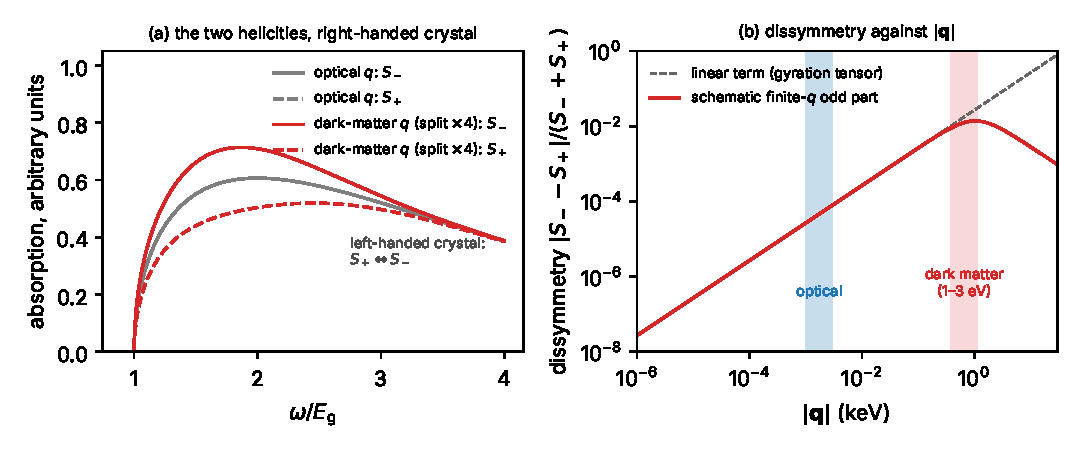
\includegraphics[width=0.95\linewidth]{figures/ch14/fig14_5.pdf}
  \caption{Circular dichroism of a chiral crystal such as tellurium. Schematic: all curves are model curves, not computed for tellurium. (a) Absorption of the two helicities, $S_\pm = S_{\mathrm{T}} \mp \hat{\vect{q}}\cdot\boldsymbol{\mathcal{G}}_{\mathrm{OA}}$ (\cref{eq:14.5-helicity}), for a model band edge at $E_{\mathrm{g}}$ in the right-handed form, at an optical momentum (gray, split invisible) and at a dark-matter momentum (red, split exaggerated four times). The left-handed form exchanges $S_+$ and $S_-$. (b) The dissymmetry against $|\vect{q}|$: the linear term $q|g|$ with $|g| = \SI{0.1}{bohr}$, the order of the computed gyration of trigonal crystals~\cite[Table~I]{zabalo2023natural} (dashed), and a schematic turnover at the inverse of a \SI{6}{\angstrom} helix pitch (red). Blue band: photons of 1 to \SI{3}{eV}; red band: the smallest dark-matter momenta at the same energies, $\omega/v_{\mathrm{max}}$. The odd part beyond the linear term is not known.}
  \label{fig:14-cd}
\end{figure}

Dark matter sees $\boldsymbol{\mathcal{G}}_{\mathrm{OA}}$ only through a coupling tensor with an antisymmetric current block. In \cref{tab:8-operators} the current row of $\mathcal{O}_5$ has the potential $\tilde V_{j^\delta} = -(\ii/m_e)c_5\epsilon_{\mu\gamma\delta}S^\mu_\chi q^\gamma$, and that of $\mathcal{O}_8$ has $\tilde V_{j^\delta} = -c_8S^\delta_\chi$. Each alone leads to a real symmetric $\mathfrak{D}_{jj}$: $\frac14|c_8|^2\delta_{\alpha\beta}$ for $\mathcal{O}_8$ and $(|c_5|^2/4m_e^2)(q^2\delta_{\alpha\beta} - q_\alpha q_\beta)$ for $\mathcal{O}_5$. Their interference, with $\Tr_\chi(S^\mu_\chi S^\nu_\chi)/2 = \delta_{\mu\nu}/4$ in \cref{eq:8.1-D}, gives
\begin{equation*}
  \mathfrak{D}_{j^\alpha j^\beta} \supset -\frac{\ii}{2m_e}\,\Real(c_5^*c_8)\,\epsilon_{\alpha\beta\gamma}q^\gamma ,
\end{equation*}
purely imaginary and antisymmetric, and its contraction with \cref{eq:14.5-GOA} is $(1/m_e)\Real(c_5^*c_8)\,\vect{q}\cdot\boldsymbol{\mathcal{G}}_{\mathrm{OA}}$. Since $\boldsymbol{\mathcal{G}}_{\mathrm{OA}}$ changes sign between enantiomers, the difference of their rates isolates this term. The density rows of $\mathcal{O}_5$ and $\mathcal{O}_8$ meet the current rows through the block $S_{nj}$. Inversion maps one enantiomer onto the other and, by \cref{eq:14.5-recip} with $\sigma^{\mathsf{P}}_n\sigma^{\mathsf{P}}_j = -1$, gives $S^{\mathrm{L}}_{nj}(\vect{q}) = -S^{\mathrm{R}}_{nj}(-\vect{q})$, so the enantiomer-odd part $S^{\mathrm{R}}_{nj}(\vect{q}) - S^{\mathrm{L}}_{nj}(\vect{q})$ is a vector even in $\vect{q}$. Averaged over crystal orientations at fixed $\vect{q}$, the enantiomer-odd part must point along $\hat{\vect{q}}$. A vector even in $\vect{q}$ cannot point along $\hat{\vect{q}}$, so the average vanishes; the enantiomer-odd part also enters contracted with $\vect{q}\times\bar{\vect{v}}_\chi$, which is orthogonal to $\hat{\vect{q}}$. Inserting the interference term in \cref{eq:8.2-spectrum} and averaging over orientations with the kernel $\eta(\vmin)/2q$ of \cref{eq:A.8-eta} gives
\begin{keyresult}[Enantiomer difference of the rate]
\begin{equation}
  \frac{\dd\mathcal{R}^{\mathrm{R}}}{\dd\omega} - \frac{\dd\mathcal{R}^{\mathrm{L}}}{\dd\omega}
  = \frac{\rho_\chi}{\mchi\,\rho_T}\int\frac{q\,\dd q}{2\pi^2}\,\eta(\vmin)\,\frac{q}{m_e}\,\Real\bigl[c_5^*(q)\,c_8(q)\bigr]\,\bar{\mathcal{G}}_{\mathrm{OA}}(q,\omega) ,
  \label{eq:14.5-enant}
\end{equation}
with $\bar{\mathcal{G}}_{\mathrm{OA}}(q,\omega)$ the average of $\hat{\vect{q}}\cdot\boldsymbol{\mathcal{G}}_{\mathrm{OA}}$ over the directions of $\vect{q}$ in the right-handed form.
\end{keyresult}
\noindent Operator $\mathcal{O}_8 = \vect{S}_\chi\cdot\vect{v}^\perp$ is odd under inversion and $\mathcal{O}_5$ is even. Only dark matter whose couplings violate parity therefore has different rates in the two enantiomers, for example a particle with both a magnetic dipole moment, which produces $\mathcal{O}_5$, and an anapole moment, which produces $\mathcal{O}_8$ (\cref{sec:8.1}). The couplings supply one parity-odd factor, and the crystal supplies the other, $\boldsymbol{\mathcal{G}}_{\mathrm{OA}}$. Because $\vect{q}\cdot\boldsymbol{\mathcal{G}}_{\mathrm{OA}}$ is even in $\vect{q}$, the enantiomer difference is not a wind asymmetry: at fixed orientation it contains the multipoles $\ell = 0$ and $\ell = 2$ of \cref{eq:11.7-rate} and modulates with the even halo multipoles. Relative to the transverse-current part of the rate of $\mathcal{O}_8$ alone, $\frac12|c_8|^2S_{\mathrm{T}}$, the interference term is the dissymmetry of \cref{eq:14.5-helicity} at dark-matter momenta times $2|c_5|q/(m_e|c_8|)$.

\begin{workedexample}{Point-group test for odd responses in $\alpha$-quartz}\label{we:14-quartz}
$\alpha$-Quartz, like tellurium, has the point group $32$ ($D_3$): the identity, two rotations by $\pm2\pi/3$ about the optic axis $\hat{\vect{z}}$, and three rotations by $\pi$ about twofold axes in the basal plane. All six are proper, $\det\mathsf{R} = 1$, and the class values of $1 + 2\cos\theta_{\mathsf{R}}$ are $3$, $0$ and $-1$ (\cref{app:C.17}).

\emph{Scalar responses.} An odd part of a scalar such as $S(\vect{q},\omega)$ starts with the harmonics $\ell = 1$, which transform as a polar vector. By \cref{eq:C.17-ninv,eq:C.17-polar} their invariants number $(3 + 2\cdot0 + 3\cdot(-1))/6 = 0$. The harmonics $\ell = 3$, with characters $\sin(\frac72\theta)/\sin(\frac12\theta) = 7$, $1$, $-1$, have $(7 + 2 - 3)/6 = 1$ invariant. Quartz keeps time reversal, however, and by \cref{eq:14.5-recip} its density response is even anyway; a magnetic crystal with the same point group could have a scalar odd part starting at $\ell = 3$, never at $\ell = 1$, because the group is not polar.

\emph{The current response.} The gyration tensor transforms with $(\det\mathsf{R})(1 + 2\cos\theta_{\mathsf{R}})^2 = 9$, $0$, $1$ on the three classes, and \cref{eq:C.17-gyration} gives $N_{\mathrm{gyr}} = (9 + 0 + 3)/6 = 2$. Projecting all nine components with $|\mathcal{P}|^{-1}\sum_{\mathsf{R}}(\det\mathsf{R})\,\mathsf{R}\otimes\mathsf{R}$ leaves the two diagonal tensors $\operatorname{diag}(1,1,0)$ and $\operatorname{diag}(0,0,1)$, so $g = \operatorname{diag}(g_{11}, g_{11}, g_{33})$. The density-functional values are $g_{11} = \SI{-0.071}{bohr}$ and $g_{33} = \SI{0.125}{bohr}$~\cite[Table~I]{zabalo2023natural}.

\emph{Consequences.} Along the optic axis, $g_{\hat q\hat q} = g_{33}$ and \cref{eq:14.5-rot} gives $\rho = \SI{21.6}{\degree.mm^{-1}}$ at \SI{2.105}{eV}. Averaged over directions, $g_{\hat q\hat q}$ becomes $(2g_{11} + g_{33})/3 = \SI{-0.0057}{bohr}$, only $-0.045$ of $g_{33}$, because $g_{11}$ and $g_{33}$ have opposite signs. If the same cancellation held for $\Imag g$ above the gap, the orientation-averaged enantiomer difference \cref{eq:14.5-enant} of quartz would be twenty times smaller than the difference for $\vect{q}$ along the optic axis. A crystal held with its axis along the wind would gain the factor of twenty back through the multipole $\ell = 2$. GaAs, with $N_{\mathrm{gyr}} = 0$ (\cref{we:C-gyration}), has no $\boldsymbol{\mathcal{G}}_{\mathrm{OA}}$ at linear order although it lacks inversion, and no enantiomers.
\end{workedexample}

\subsection{Chiral phonons}\label{sec:14.5-phonons}

In GaAs, which lacks inversion, the atoms in a phonon of a general wavevector move on ellipses, and a phonon of the lowest band carries on average $0.12$ units of angular momentum. In the normalization of \cref{eq:5.3-u}, the angular momentum of mode $\vect{Q}\nu$ in units of $\hbar$ is
\begin{equation}
  \vect{L}^{\mathrm{ph}}_{\vect{Q}\nu} = \sum_\kappa\vect{L}^{\mathrm{ph}}_{\kappa,\vect{Q}\nu}, \qquad
  \vect{L}^{\mathrm{ph}}_{\kappa,\vect{Q}\nu} = -\ii\,\vect{e}_{\kappa\nu}(\vect{Q})^*\times\vect{e}_{\kappa\nu}(\vect{Q}) ,
  \label{eq:14.5-Lph}
\end{equation}
the definition of Romao and collaborators and of Matas, Krizek and Romao~\cites[Eq.~(6)]{romao2023chiral}[Eq.~(11)]{matas2025chiral}. Each term is real, and $|\vect{L}^{\mathrm{ph}}_{\vect{Q}\nu}| \le \sum_\kappa|\vect{e}_{\kappa\nu}|^2 = 1$, with equality for circular motion. Time reversal gives $\vect{e}_{\kappa\nu}(-\vect{Q}) = \vect{e}_{\kappa\nu}(\vect{Q})^*$ for a nondegenerate mode, so $\vect{L}^{\mathrm{ph}}_{-\vect{Q}\nu} = -\vect{L}^{\mathrm{ph}}_{\vect{Q}\nu}$. Inversion maps the axial vector $\vect{L}^{\mathrm{ph}}$ at $\vect{Q}$ onto itself at $-\vect{Q}$, and with both time reversal and inversion $\vect{L}^{\mathrm{ph}}$ vanishes, as in silicon. In a magnetically ordered crystal any phonon can carry angular momentum.

The angular momentum labels the final state, and the coupling is the density coupling of \cref{eq:11.1-S1}, which creates mode $\vect{Q}\nu$ with the amplitude given there. Multiplying each term of the one-phonon response \cref{eq:11.1-S1} by $\delta^3(\vect{L} - \vect{L}^{\mathrm{ph}}_{\vect{Q}\nu})$ gives the final-state-resolved one-phonon response $S^{(1)}_A(\vect{q},\omega;\vect{L})$, whose integral over $\vect{L}$ is $S^{(1)}_A(\vect{q},\omega)$. With $S^{(1)}_A$ even in $\vect{q}$ and $\vect{L}^{\mathrm{ph}}$ odd, the mean angular momentum of the created phonons survives the integration over $\vect{q}$ only through the part of the halo kernel odd in $\hat{\vect{q}}\cdot\hat{\vect{v}}_{\mathrm{E}}$, the odd multipoles of \cref{eq:11.7-ups}. To first order in $\hat{\vect{v}}_{\mathrm{E}}$ the mean angular momentum is $\langle L_i\rangle = G_{ij}\hat v_{\mathrm{E},j}$, and the crystal tensor $G_{ij}$ joins an axial index to a polar one, like the gyration tensor. The invariants of $G_{ij}$ are counted by \cref{eq:C.17-gyration}: in GaAs there are none, so the phonons that dark matter creates there carry no net angular momentum along the wind at this order, while $\alpha$-quartz and tellurium allow two constants (\cref{we:14-quartz}).

Chiral phonons are detected through their magnetic moment. A nucleus of Born charge $eZ^*_\kappa$ on a closed orbit has the moment $(eZ^*_\kappa/2M_\kappa)\,\vect{u}\times\vect{P}$. Summed over the nuclei, the moment operator is bilinear in the phonon operators, has no matrix element between the ground state and one phonon, and measures a property of the occupied mode. In a state with one phonon in mode $\vect{Q}\nu$,
\begin{equation}
  \boldsymbol{\mu}^{\mathrm{ph}}_{\vect{Q}\nu} = \sum_\kappa\frac{eZ^*_\kappa}{2M_\kappa}\,\vect{L}^{\mathrm{ph}}_{\kappa,\vect{Q}\nu} ,
  \label{eq:14.5-muph}
\end{equation}
which is the moment of Refs.~\cites[Eq.~(7)]{romao2023chiral}[Eq.~(12)]{matas2025chiral} for isotropic Born charges. With the PBE Born charges of \cref{sec:5.5}, $Z^* = \pm2.09$, GaAs reaches at most $0.015\,\mu_N$ in its lowest band, and no mode exceeds $Z^*_{\mathrm{Ga}}m_p/M_{\mathrm{Ga}} = 0.030\,\mu_N$, which a mode with $|\vect{L}^{\mathrm{ph}}| = 1$ on the gallium sublattice alone would have; $\mu_N$ is the nuclear magneton, $1/1836$ of $\mu_B$. Phonon moments of order $\mu_B$ have been reported in some $4f$ paramagnets and topological semimetals~\cite[Sect.~II]{romao2023chiral}. They are larger than \cref{eq:14.5-muph} by four to five orders of magnitude and come from the coupling of the lattice to the orbital and spin moments of the electrons, which the Born charge does not contain; computing them needs the derivatives of the crystal-field states with respect to the atomic displacements, separately for the spin and the orbital moment (\cref{app:E.19}). A coupling to the ionic current, such as that of a particle with a magnetic dipole moment, creates single phonons through the transverse part of that current, at first order in $q$, and not through $\boldsymbol{\mu}^{\mathrm{ph}}$.

The detector that Romao and collaborators propose reads out phonons of the lowest band, the only band whose phonons live for microseconds or longer~\cite[Sect.~III]{matas2025chiral}, after the phonons created by the dark matter have decayed into the lowest band. A phonon Hall effect, the transverse deflection of a heat current carried by chiral phonons, collects them at the surfaces, where magnetometers sense their moments~\cite[Sect.~IV]{romao2023chiral}. The rate is the one-phonon rate~\cite[Eqs.~(3), (4)]{matas2025chiral}, \cref{eq:11.1-S1} in \cref{eq:8.2-spectrum}, times a detection probability that Matas and collaborators take as the average of $|\vect{L}^{\mathrm{ph}}|$ over the lowest band, with each event ending as one phonon placed at random in that band. They quote 0.22 for LiNbO$_3$ and 0.16 for the framework CuCl(pyrimidine)~\cite[Sect.~III]{matas2025chiral}, and Romao and collaborators 0.15 for InF$_3$(4,4$'$-bipyridine)~\cite[Sect.~VII]{romao2023chiral}. The estimate assumes that each created phonon lands at random in the band, as in the average, and that its chirality survives the decay. \Cref{lim:14.5a}a tests the first assumption in GaAs. The survival of the chirality is not protected, since $L^{\mathrm{ph}}_z$ is not conserved. For $H = \frac12\vect{p}\cdot\vect{p} + \frac12\vect{u}\cdot D\vect{u}$ in mass-weighted coordinates and $L_z = \vect{u}\cdot J_z\vect{p}$, with $J_z$ the generator of rotations about $\hat{\vect{z}}$ acting on the displacement of each site, $[H, L_z] = \frac{\ii}{2}\,\vect{u}\cdot[J_z, D]\,\vect{u}$, which vanishes only if the force constants are isotropic about every site. A crystal conserves only the pseudo-angular momentum of its discrete rotations, the eigenvalue of a rotation by $2\pi/n$ defined modulo $n$, and the anharmonic decay changes $\vect{L}^{\mathrm{ph}}$. The probability that a created phonon ends as a detectable chiral phonon is the solution of a linear system over the three-phonon decay rates, $\boldsymbol{\mathcal{N}}^{\mathrm{ch}} = (\mathbb{1} - \mathsf{M})^{-1}\vect{b}$, with the angular momentum recomputed for each daughter.

\subsection{Single-molecule magnets}\label{sec:14.5-smm}

The twelve manganese ions of a Mn$_{12}$-acetate molecule lock into a total spin $|\vect{S}| = 10$, held along the molecular axis by an axial anisotropy. Electron spin resonance measures $D = \SI{0.454}{cm^{-1}} = \SI{0.0563}{meV}$ and a quartic term $B_4^0 = \SI{-2.0e-5}{cm^{-1}}$~\cite[Fig.~2]{edwards2003evidence}, so that in a field along the axis the molecule has
\begin{equation}
  H_{\mathrm{mol}} = -D\,S_z^2 + B_4^0\,O_4^0 - \omega_{\mathrm{Lar}}S_z ,
  \label{eq:14.5-Hmol}
\end{equation}
with the axial term $-DS_z^2$ of Alves and collaborators~\cite[Eq.~(3)]{alves2026search}, the quartic operator $O_4^0 = 35S_z^4 - [30|\vect{S}|(|\vect{S}| + 1) - 25]S_z^2 + \text{const}$ of Edwards and collaborators~\cite{edwards2003evidence}, and the Zeeman term of \cref{sec:14.3-larmor}. The levels $m = -|\vect{S}|, \dots, |\vect{S}|$ form two wells separated by a barrier; at \SI{1}{T} the top of the barrier lies at $m = -1$, \SI{4.6}{meV} (\SI{53}{K}) above $m = -|\vect{S}|$. If a crystal is cooled in a field and the field is then reversed, the crystal keeps its molecules in the upper well, at $m = -|\vect{S}|$, for the relaxation time $\tau_{\mathrm{R}} \approx \tau_0\exp[(U - \frac12\Delta E_{\mathrm{Zee}})/T]$ of thermal activation over the barrier~\cite[Eq.~(4)]{alves2026search}. The molecules then store the Zeeman energy $\Delta E_{\mathrm{Zee}}$, and a local deposit of heat can release the stored energy in a front that propagates through the crystal. The propagating front, a magnetic avalanche, is the readout proposed by Alves and collaborators.

The molecules lie far apart in their crystal, and we treat them as independent, with number density $\nd_{\mathrm{mol}}$, populations $p_m$, and the spin row $\vect{s}_e(0) = \lambda_S\sum\vect{S}$ of \cref{eq:14.3-s0}, $\lambda_S = 1$ for manganese ions with quenched orbital moments. With $s_{e,x} = \lambda_S(S^+ + S^-)/2$ and $|\langle m \pm 1|S^\pm|m\rangle|^2 = |\vect{S}|(|\vect{S}| + 1) - m(m \pm 1)$, \cref{eq:4.2-Sab} gives
\begin{equation}
  \begin{split}
  S_{xx}(0,\omega) = \frac{\pi\nd_{\mathrm{mol}}\lambda_S^2}{2}\sum_mp_m\Bigl\{&\bigl[|\vect{S}|(|\vect{S}| + 1) - m(m + 1)\bigr]\delta(\omega - \omega_{m,m+1}) \\
  &+ \bigl[|\vect{S}|(|\vect{S}| + 1) - m(m - 1)\bigr]\delta(\omega - \omega_{m,m-1})\Bigr\} ,
  \end{split}
  \label{eq:14.5-smm}
\end{equation}
with $\omega_{m,m'} = E_{m'} - E_m$ the level differences of \cref{eq:14.5-Hmol}, and $S_{yy} = S_{xx}$. Without the quartic term, $\omega_{m,m+1} = -D(2m + 1) - \omega_{\mathrm{Lar}}$. A molecule in the lower well, $m = |\vect{S}|$, absorbs through $S^-$ at $D(2|\vect{S}| - 1) + \omega_{\mathrm{Lar}}$. A molecule held at $m = -|\vect{S}|$ absorbs through $S^+$ at
\begin{equation}
  \omega_{\mathrm{meta}} = D\,(2|\vect{S}| - 1) - \omega_{\mathrm{Lar}} ,
  \label{eq:14.5-meta}
\end{equation}
with the weight $2|\vect{S}|$: the metastable line, which the field moves down by \SI{0.116}{meV} per tesla while it moves the line of the lower well up. For Mn$_{12}$-acetate, $D(2|\vect{S}| - 1) = \SI{1.07}{meV}$; the quartic term raises the zero-field line to \SI{1.21}{meV}, and at \SI{1}{T} the metastable line is at \SI{1.098}{meV}, \SI{12.7}{K}. The next line of the upper well, from $m = -9$, lies \SI{0.18}{meV} lower. As for the Larmor line, the spin algebra fixes the total: summed over all lines of a well, the net absorptive weight $\sum_m(p_m - p_{m+1})[|\vect{S}|(|\vect{S}| + 1) - m(m + 1)]$ is $2|\langle S_z\rangle|$, however the population is spread.

An axion-like particle reaches the line through \cref{eq:14.3-abs}, with $p_\phi^2$ replaced by its component perpendicular to the molecular axis, and a dark photon through its magnetic field, as in \cref{sec:14.3}. The electric field of a dark photon couples instead to the electronic and vibrational dipoles of the molecules. The rate through the electric field is the absorption rate of \cref{sec:8.2-absorption} with the mixing of \cref{eq:8.4-zetaeff}, $\zeta^2\sigma_1/|\varepsilon|^2$, with $\sigma_1 = n_r\alpha$ from the measured absorption coefficient $\alpha(\omega)$ of the crystal~\cite[Eqs.~(9), (10)]{alves2026search}. An axion-like particle in a static field is a dark photon with $\zeta = g_{a\gamma\gamma}B_0/m_\phi$ (\cref{eq:10.7-alpB}), with a rate quadratic in $g_{a\gamma\gamma}B_0$. The avalanche needs a deposit of about \SI{e-2}{eV} in molecules of radius 2 to \SI{3}{nm}~\cite[Eq.~(6), Fig.~6]{alves2026search}; an absorbed boson deposits its whole energy $\omega_\phi \simeq m_\phi$, and for any nonrelativistic speed the trigger is a condition on $m_\phi$ alone. For $m_\phi \ge \SI{e-2}{eV}$ halo absorption triggers with the full halo density, below \SI{e-2}{eV} halo absorption cannot trigger, and a boosted population would need its own energy spectrum.

\Cref{lim:14.5a} compares the two simple descriptions, the band average of $|\vect{L}^{\mathrm{ph}}|$ and the full weight $2|\vect{S}|$ of the metastable line, with the final-state-resolved responses. In GaAs the average of $|\vect{L}^{\mathrm{ph}}|$ over the lowest band is 0.124 with the force constants of \cref{sec:5.5}. Scaling the long-range dipole part of the force constants between zero and 1.5 times its value moves the band average between 0.175 and 0.107, within $\pm\SI{40}{\percent}$. Weighted with the one-phonon rate, the average over the lowest-band phonons that dark matter creates directly approaches 0.112, within \SI{10}{\percent} of the band average, for $\mchi \ge \SI{2.2}{MeV}$, where these phonons carry \SI{30}{\percent} of the one-phonon rate. Below \SI{0.8}{MeV} the lowest band takes less than \SI{1}{\percent} of the rate, and all created phonons together carry on average less than $0.03$ below \SI{0.2}{MeV}, because the long-wavelength acoustic phonons that a light particle can create move their atoms almost on straight lines. For light dark matter the detected chirality is thus set by the decay. For the molecular magnet the simple picture, every molecule in $m = -|\vect{S}|$, gives the full line weight $2|\vect{S}|$. Thermal population of the upper well lowers the weight of the line at $\omega_{\mathrm{meta}}$ by stimulated emission and moves it to the neighboring lines. The line keeps \SI{90}{\percent} of $2|\vect{S}|$ for $\omega_{\mathrm{meta}}/T \ge 3.0$, that is below \SI{4.2}{K} for Mn$_{12}$-acetate at \SI{1}{T}.

\begin{limitbox}[Chiral phonons and molecular magnets][lim:14.5a]
(a) Probability of a detectable chiral phonon taken as the average of $|\vect{L}^{\mathrm{ph}}|$, \cref{eq:14.5-Lph}, over the lowest band, applied to the one-phonon rate~\cites[Eqs.~(6), (7)]{romao2023chiral}[Eqs.~(3), (4), (11), (12)]{matas2025chiral}. (b) Metastable line of a molecular magnet held in $m = -|\vect{S}|$, at $\omega_{\mathrm{meta}}$ of \cref{eq:14.5-meta} with weight $2|\vect{S}|$~\cite[Eqs.~(3), (4)]{alves2026search}.
\par\smallskip
{\centering
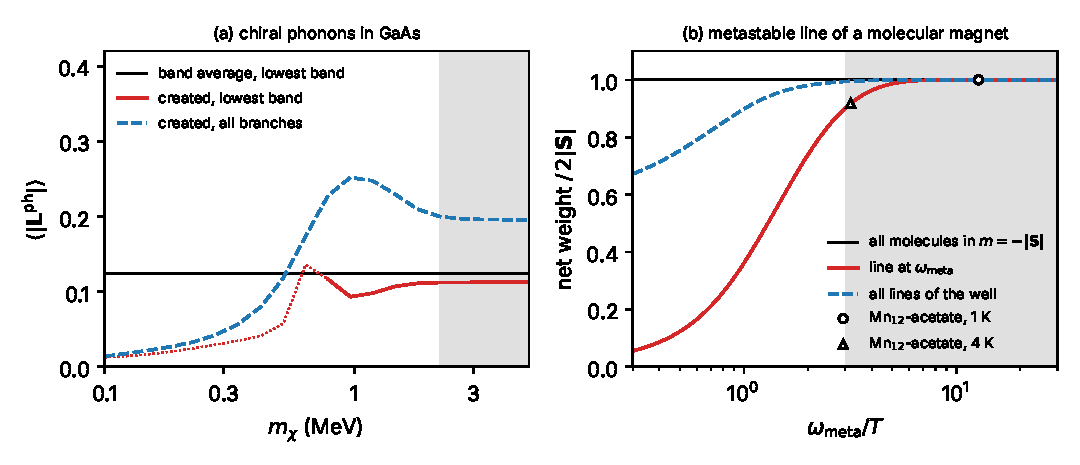
\includegraphics[width=0.98\linewidth]{figures/ch14/limit14_5a.pdf}
\captionof{figure}{(a) GaAs, from the PBE force constants of \cref{sec:5.5}. Black: the average of $|\vect{L}^{\mathrm{ph}}|$ over the lowest band, 0.124. Red: the same average weighted with the one-phonon rate of a heavy mediator coupled to nucleon number (\cref{eq:11.1-S1}, orientation-averaged halo kernel, $T = 0$), for the lowest-band phonons that the dark matter creates directly, against $\mchi$; dotted where the lowest band takes less than \SI{1}{\percent} of the rate. Blue dashed: the same for all created phonons. Gray: red within \SI{10}{\percent} of black, $\mchi \ge \SI{2.2}{MeV}$. (b) Mn$_{12}$-acetate ($|\mathbf{S}| = 10$, $D = \SI{0.454}{cm^{-1}}$, $B_4^0 = \SI{-2.0e-5}{cm^{-1}}$, \SI{1}{T}, $g_{\mathrm{ion}} = 2$, $\omega_{\mathrm{meta}} = \SI{1.098}{meV}$): net absorptive weight over $2|\mathbf{S}|$ against $\omega_{\mathrm{meta}}/T$, for thermal populations inside the upper well. Red: the line at $\omega_{\mathrm{meta}}$; blue dashed: all lines of the well, $2|\langle S_z\rangle|/2|\mathbf{S}|$. Gray: the line within \SI{10}{\percent} of $2|\mathbf{S}|$, $\omega_{\mathrm{meta}}/T \ge 3.0$. Markers: \SI{1}{K} and \SI{4}{K}.}\label{fig:14-limit-chiral}
\par}
\smallskip
Outside the gray regions the band average misstates the chirality of the phonons that a light particle creates, and a warm molecular crystal spreads the metastable weight over the lines of its well.
\end{limitbox}

\subsection{Magnetoelectric response of multiferroics}\label{sec:14.5-mf}

Hexagonal Lu$_{1-x}$Sc$_x$FeO$_3$ with $x \approx 0.4$ becomes ferroelectric at about \SI{1200}{K}. Below its magnetic ordering temperature $T_{\mathrm{CM}} \approx \SI{160}{K}$ the canted spins of its iron ions add a net magnetization parallel to the polarization. For hexagonal LuFeO$_3$ ($x = 0$), density-functional calculations give a polarization of \SI{10.5}{\micro C.cm^{-2}} along the $c$ axis and a net moment of $0.02\,\mu_B$ per iron~\cite[Sect.~IV\,A]{roising2021axion}. A crystal with both orders breaks inversion and time reversal and keeps their product. R{\o}ising and collaborators propose that an axion field shifts the magnetization of a multiferroic with both orders through the coupling of the axion to the electron, $\delta E = -\ii g_{aee}(\partial_t\phi/2m_e^2)\langle\boldsymbol{\sigma}\cdot\nabla\rangle$~\cite[Eq.~(5)]{roising2021axion}. With $\vect{p} = -\ii\nabla$ and $\boldsymbol{\sigma} = 2\vect{S}$, the spin current of \cref{eq:8.1-rows} at $\vect{q} = 0$ is $\mathcal{J}^{\alpha\alpha}_e(0) = \sum_j\vect{p}_j\cdot\vect{S}_j/m_e = -\ii\sum_j\boldsymbol{\sigma}_j\cdot\nabla_j/2m_e$, so the coupling is $(g_{aee}/m_e)(\partial_t\phi)\,\mathcal{J}^{\alpha\alpha}_e(0)$, the second term of \cref{eq:8.1-alp} at $\vect{p}_\phi \to 0$. By the Kubo formula of \cref{sec:4.2}, the spin density then responds as
\begin{equation}
  \frac{\delta\langle s^z_e(0)\rangle(\omega)}{\Vol} = \frac{g_{aee}}{m_e}\,R_{s^z\mathcal{J}}(0,\omega)\,(\partial_t\phi)(\omega) = -\ii\,\frac{g_{aee}m_\phi}{m_e}\,R_{s^z\mathcal{J}}(0,m_\phi)\,\phi(\omega) ,
  \label{eq:14.5-cross}
\end{equation}
with $R_{s^z\mathcal{J}}$ the retarded response of $s^z_e$ to $\mathcal{J}^{\alpha\alpha}_e$ and the magnetization $-2\mu_B$ times the left-hand side. The spin-density and spin-current rows have opposite signs under both time reversal and inversion, $\sigma^{\mathsf{T}}_s\sigma^{\mathsf{T}}_{\mathcal{J}} = \sigma^{\mathsf{P}}_s\sigma^{\mathsf{P}}_{\mathcal{J}} = -1$, so by \cref{eq:14.5-recip} inversion removes the block at $\vect{q} = 0$ and time reversal removes its symmetric part, the part that survives as $\omega \to 0$. The adiabatic response thus needs both symmetries broken, as in Lu$_{1-x}$Sc$_x$FeO$_3$ below $T_{\mathrm{CM}}$.

The Lehmann form of \cref{sec:4.2}, $R_{ab} = \Vol^{-1}\sum_{i,n}(p_i - p_n)\langle i|O_a^\dagger|n\rangle\langle n|O_b|i\rangle/(\omega - \omega_{ni} + \ii0^+)$, shows which states contribute. Far below $T_{\mathrm{CM}}$ the states $n$ reached at $\vect{q} = 0$ from the ordered state are its uniform magnon modes, in linear spin-wave theory as in \cref{sec:14.3}. Each mode $\nu$ with both matrix elements nonzero contributes a pair of poles at $\pm\omega_\nu$, which combine for real matrix elements into a term proportional to $2\omega_\nu/(\omega^2 - \omega_\nu^2)$. Two conditions restrict the modes. If the Hamiltonian conserves the total spin component $S^z_{\mathrm{tot}}$ and $s^z_e(0) = \lambda_SS^z_{\mathrm{tot}}$, then $s^z_e(0)$ has no time dependence and $R_{s^z\mathcal{J}}(0,\omega)$ vanishes at every $\omega \ne 0$. The response needs a spin--orbit coupling, a Dzyaloshinskii--Moriya interaction or a single-ion anisotropy that does not commute with $S^z_{\mathrm{tot}}$, such as the one that cants the spins of hexagonal Lu$_{1-x}$Sc$_x$FeO$_3$. And $\mathcal{J}^{\alpha\alpha}_e$ is odd under inversion, and it has matrix elements within the ground configuration of an ion only through a crystal field without inversion together with spin--orbit coupling (\cref{sec:14.3}). The response is thus at least of second order in spin--orbit coupling: one order for the vertex, and one or two for the breaking of $S^z_{\mathrm{tot}}$, by a Dzyaloshinskii--Moriya term or a single-ion term.

Far below $T_{\mathrm{CM}}$, where thermal magnons reduce the moment by less than \SI{10}{\percent} ($T \le 0.37\,T_{\mathrm{CM}}$ for spin $\frac52$ with nearest-neighbor exchange on a simple-cubic lattice), the Lehmann sum over the uniform magnons and their thermal population is the controlled result. Near $T_{\mathrm{CM}}$, dynamic scaling predicts the structure $R_{s^z\mathcal{J}}(0,\omega;T) = \chi_\times(T)\,\Phi(\omega\tau(T))$, with a relaxation time $\tau \propto |T - T_{\mathrm{CM}}|^{-\nu z}$, $\nu$ the correlation-length exponent and $z$ the dynamic exponent~\cite[Sect.~III\,D]{roising2021axion}; the amplitude $\chi_\times$ and the scaling function $\Phi$ of a real material are not known. The exchange, Dzyaloshinskii--Moriya and anisotropy constants of the spin model for $T \ll T_{\mathrm{CM}}$ come from DFT~$+\,U$ energy mappings, with spin--orbit coupling included for the vertex of $\mathcal{J}^{\alpha\alpha}_e$.

\subsection{Uncertainty budget of the magnetic rates}\label{sec:14.5-budget}

\Cref{tab:14-nuisances} collects the truncations and inputs of the chapter with their sizes. Near the lightest masses the anisotropy row dominates every other row by more than an order of magnitude, and it is a model, not a calculation. For absorption into the uniform mode, the shape of the sample and the width of the line set the rate, and neither depends on the spin-wave expansion. In the coherent regime the largest effects are statistical: the length of the record against $t_{\mathrm{coh}}$ and $T_2$, and whether the likelihood contains the random amplitude.
\begin{table}[tbp]
  \caption{Uncertainty budget of the magnetic rates and of the coherent regime. Classes as in \cref{tab:10-nuisances}; ``unsized'' marks an item with no size known. Sizes are for NiO, YIG, MnF$_2$, GaAs, Mn$_{12}$-acetate and $^{207}$Pb in PMN-PT as named.}
  \label{tab:14-nuisances}
  \centering\scriptsize\setlength{\tabcolsep}{3pt}
  \begin{tabular}{@{}>{\raggedright\arraybackslash}p{0.27\linewidth}>{\raggedright\arraybackslash}p{0.13\linewidth}>{\raggedright\arraybackslash}p{0.48\linewidth}>{\raggedright\arraybackslash}p{0.08\linewidth}@{}}
    \toprule
    Truncation or input & Type & Size & Section \\
    \midrule
    One-magnon weight of linear spin-wave theory & normali\-zation & high by about $\Delta S/|\vect{S}|$: \SI{7.8}{\percent} (NiO), \SI{3.1}{\percent} for $|\vect{S}| = \frac52$, \SI{16}{\percent} for $|\vect{S}| = \frac12$ & \cref{sec:14.1} \\
    Two-magnon continuum & new support & 0.073 of the one-magnon weight over the zone (NiO); $w_\parallel/w_\perp < 0.05$ below \SI{0.5}{keV} & \cref{sec:14.2} \\
    Final-state interaction of the pair & tilt; new support & about 0.04 of the spin response, moved in energy (NiO); bound pair unsized & \cref{sec:14.2} \\
    Magnetic anisotropy near the gap & threshold; tilt in $\mchi$ & NiO, \SI{5}{meV} threshold, one-constant gap \SI{4.54}{meV}: rate $\times29$ at \SI{10}{keV} (upper value), $\times1.35$ at \SI{30}{keV}, $< \SI{3}{\percent}$ above \SI{100}{keV} & \cref{sec:14.1} \\
    Exchange constants from DFT~$+\,U$ & threshold & $J_2$ of NiO 11 to \SI{27}{meV} against 19.01: magnon energies $\times0.58$ to 1.42 & \cref{sec:14.1} \\
    Magnon--phonon mixing & tilt & gap \SI{3.0}{\percent} of the crossing energy at \SI{2.83}{GHz} (YIG model); NiO unsized & \cref{sec:14.2} \\
    Thermal magnons & new support & $\ee^{-\omega_{\mathrm{gap}}/T}$, exponent $-5\times10^3$ at \SI{10}{mK} (NiO) & \cref{sec:14.1} \\
    Sample shape & threshold; normali\-zation & YIG film within \SI{10}{\percent} of the Larmor line for $B_0 \ge 4.8\,\mu_0M_{\mathrm{s}}$; weight $\times1.74$ at \SI{10}{\micro eV}; saturated sphere exact & \cref{sec:14.3} \\
    Zero-point correction to the resonance weight & normali\-zation & 5 to \SI{23}{\percent} for $|\vect{S}| = \frac32$, $\omega_A/\omega_E = 2$ to 0.3; MnF$_2$ unsized & \cref{sec:14.3} \\
    Resonance of MnF$_2$ & threshold & fitted fields \SI{7}{\percent} below the measured \SI{1.1}{meV} and \SI{9.4}{T}; peak rate unchanged & \cref{sec:14.3} \\
    Width $\varGamma_{\mathrm{M}}$ of the uniform line & normali\-zation & peak rate $\propto 1/\varGamma_{\mathrm{M}}$; $10^{-5}\omega$ for YIG assumed & \cref{sec:14.3} \\
    Spin fraction $\lambda_S$ of quenched $3d$ ions & normali\-zation & $1 - O(\xi_{\mathrm{ion}}^2/\Delta_{\mathrm{CF}}^2)$ & \cref{sec:14.3} \\
    In-medium mixing of a dark photon & normali\-zation & set by the dielectric constant and the enclosure; unsized & \cref{sec:14.3} \\
    Neutron data for quenched ions & normali\-zation & $[\lambda_S/(g_{\mathrm{ion}}/2)]^2 = 0.83$ (Ni$^{2+}$, $g_{\mathrm{ion}} = 2.2$) or 0.73 (2.34); 0.973 at \SI{5.3}{keV} & \cref{sec:14.4} \\
    Longitudinal response from neutron data & new support & needs the localized-moment form or the isotropy hypothesis & \cref{sec:14.4} \\
    Record length against $t_{\mathrm{coh}}$ and $1/\varGamma_{\mathrm{tg}}$ & normali\-zation & mean within \SI{10}{\percent} of the golden rule for $t_{\mathrm{int}} \ge 13\,t_{\mathrm{coh}}$ ($T_2 \to \infty$) to $t_{\mathrm{coh}}$ ($T_2 = 0.1\,t_{\mathrm{coh}}$) & \cref{sec:14.6} \\
    Field amplitude fixed instead of Rayleigh & normali\-zation & limit too strong by 1.99 below $t_{\mathrm{coh}}$, 1.015 at $100\,t_{\mathrm{coh}}$; 2.73 at the detection threshold & \cref{sec:14.6} \\
    Linearized Bloch equation & normali\-zation & $(\Omega_{\mathrm{Rabi}}t)^2/6$ in the transient; \SI{30}{\percent} saturation at the PMN-PT threshold & \cref{sec:14.6} \\
    Inhomogeneous broadening; effective field $E^*$ & normali\-zation & $u_{\mathrm{sp}} = 3.8\times10^{-4}$; $E^*$ about \SI{50}{\percent} ($^{207}$Pb in PMN-PT) & \cref{sec:14.6} \\
    Line shape of the halo & tilt & standard halo only; unsized & \cref{sec:14.6} \\
    Chiral phonons as a band average & normali\-zation & GaAs 0.124, $\pm\SI{40}{\percent}$ with the dipole part of the force constants; rate-weighted within \SI{10}{\percent} only for $\mchi \ge \SI{2.2}{MeV}$; decay branching unsized & \cref{sec:14.5} \\
    Upper-well population of a molecular magnet & normali\-zation & Mn$_{12}$-acetate at \SI{1}{T}: line keeps \SI{90}{\percent} of $2|\vect{S}|$ below \SI{4.2}{K} & \cref{sec:14.5} \\
    Multiferroic response near $T_{\mathrm{CM}}$ & normali\-zation; tilt & unsized & \cref{sec:14.5} \\
    \bottomrule
  \end{tabular}
\end{table}
